\begin{center}
    {\LARGE \textbf{2017物理化学}} \\[2ex]
    {\large 时量180分钟 \quad 满分150分}
\end{center}

\vspace{0.5cm}
\noindent\textbf{注意事项:}
\begin{enumerate}[label=\arabic*., parsep=0pt, itemsep=0pt]
    \item 答题前,考生先将自己的姓名、学号、考场号、座位号填写在答题卡上,将条形码准确粘贴在考生信息条形码粘贴区。
    \item 考试结束后,将本试卷与答题纸一并收回。
    \item 回答各个问题时,将答案写在答题纸上,写在本试卷上无效。
\end{enumerate}

\vspace{0.5cm}
\noindent\textbf{一、选择题（30 pts.）}

\begin{enumerate}[label=\arabic*., itemsep=1.5ex]
    \item 有一容器四壁导热，上部有一可移动的活塞，在该容器中同时放入锌块和盐酸，发生化学反应后活塞将上移一定距离，若以锌和盐酸为体系则
    \begin{tasks}(2)
        \task $Q<0$，$W=0$，$\Delta_\mathrm{r}U<0$
        \task $Q=0$，$W>0$，$\Delta_\mathrm{r}U<0$
        \task $Q<0$，$W>0$，$\Delta_\mathrm{r}U=0$
        \task $Q<0$，$W>0$，$\Delta_\mathrm{r}U<0$
    \end{tasks}
    \item 在HAc解离常数测定的实验中，直接测定的物理量是不同浓度的HAc溶液的
    \begin{tasks}(4)
        \task 电导率
        \task 电阻
        \task 摩尔电导率
        \task 解离度
    \end{tasks}
    \item 体系经历一个正的卡诺循环后，试判断下列哪一种说法是错误的？
    \begin{tasks}(1)
        \task 体系本身没有任何变化
        \task 再沿反方向经历一个可逆的卡诺循环，最后体系和环境都没有任何变化
        \task 体系复原了，但环境并未复原
        \task 体系和环境都没有任何变化
    \end{tasks}
    \item 下面哪一个公式表示了离子独立移动定律
    \begin{tasks}(2)
        \task $\alpha = \Lambda_\mathrm{m}/\Lambda_\mathrm{m}^\infty$
        \task $\lambda_\mathrm{m,+}^\infty = t_+^\infty \Lambda_\mathrm{m}^\infty$
        \task $\lambda_\mathrm{m,+}^\infty = \Lambda_\mathrm{m}^\infty - \lambda_\mathrm{m,-}^\infty$
        \task $\Lambda_\mathrm{m} = k/c$
    \end{tasks}
    \item 一理想气体化学反应的平衡常数与其标准吉布斯自由能变化（$\Delta_\mathrm{r}G_\mathrm{m}^\ominus$）的关系有：
    
    (1) $K_p^\ominus = \exp(-\Delta_\mathrm{r}G_\mathrm{m}^\ominus/RT)$

    (2) $K_c^\ominus = \exp(-\Delta_\mathrm{r}G_\mathrm{m}^\ominus/RT)$

    (3) $K_x = \exp(-\Delta_\mathrm{r}G_\mathrm{m}^\ominus/RT)$
    
    下述说法正确的是
    \begin{tasks}(2)
        \task (1)、(2)和(3)式均正确
        \task (1)式正确
        \task (2)式正确
        \task (3)式正确
    \end{tasks}
    \item 在$1100^\circ\mathrm{C}$时，发生下列反应：
    
    (1) $\ce{C(s) + 2S(s) = CS2(g)}$ \quad $K_1=0.258$

    (2) $\ce{Cu2S(s) + H2(g) = 2Cu(s) + H2S(g)}$ \quad $K_2=3.9\times10^{-3}$

    (3) $\ce{2H2S(g) = 2H2(g) + 2S(s)}$ \quad $K_3=2.29\times10^{-2}$

    则$1100^\circ\mathrm{C}$时反应 $\ce{C(s) + 2Cu2S(s) = 4Cu(s) + CS2(g)}$ 的$K$为
    \begin{tasks}(4)
        \task $8.99\times10^{-8}$
        \task $8.99\times10^{-5}$
        \task $3.69\times10^{-5}$
        \task $3.69\times10^{-8}$
    \end{tasks}
    \item $\ce{NaCl}$稀溶液的摩尔电导率$\Lambda_\mathrm{m}$与$\ce{Na+}$、$\ce{Cl-}$离子的淌度($U_\mathrm{i}$)之间的关系为
    \begin{tasks}(2)
        \task $\Lambda_\mathrm{m}=U_+ + U_-$
        \task $\Lambda_\mathrm{m}=U_+/F + U_-/F$
        \task $\Lambda_\mathrm{m}=U_+F + U_-F$
        \task $\Lambda_\mathrm{m}=2(U_+ + U_-)$
    \end{tasks}
    \item 已知：$\ce{Zn(s) + 1/2O2 -> ZnO}$ \quad $\Delta_\mathrm{c}H_\mathrm{m}=351.5\ \mathrm{kJ\cdot mol^{-1}}$
    $\ce{Hg(l) + 1/2O2 -> HgO}$ \quad $\Delta_\mathrm{c}H_\mathrm{m}=90.8\ \mathrm{kJ\cdot mol^{-1}}$
    因此 $\ce{Zn + HgO -> ZnO + Hg}$ 的$\Delta_\mathrm{r}H_\mathrm{m}$是
    \begin{tasks}(4)
        \task $442.2\ \mathrm{kJ\cdot mol^{-1}}$
        \task $260.7\ \mathrm{kJ\cdot mol^{-1}}$
        \task $-62.3\ \mathrm{kJ\cdot mol^{-1}}$
        \task $-442.2\ \mathrm{kJ\cdot mol^{-1}}$
    \end{tasks}
    \item 在$400\ \mathrm{K}$时，液体$\ce{A}$的蒸气压为$4\times10^4\ \mathrm{Pa}$，液体$\ce{B}$的蒸气压为$6\times10^4\ \mathrm{Pa}$，两者组成理想溶液，平衡时在液相中$\ce{A}$的摩尔分数为$0.6$。则在气相中$\ce{B}$的摩尔分数为
    \begin{tasks}(4)
        \task $0.31$
        \task $0.40$
        \task $0.50$
        \task $0.60$
    \end{tasks}
    \item 同一个反应在相同反应条件下未加催化剂时平衡常数及活化能为$k$及$E_\mathrm{a}$，加入正催化剂后则为$k'$、$E_\mathrm{a}'$，则存在下述关系
    \begin{tasks}(2)
        \task $k'=k$，$E_\mathrm{a}=E_\mathrm{a}'$
        \task $k'\neq k$，$E_\mathrm{a}\neq E_\mathrm{a}'$
        \task $k'=k$，$E_\mathrm{a}>E_\mathrm{a}'$
        \task $k'<k$，$E_\mathrm{a}'<E_\mathrm{a}$
    \end{tasks}
    \item 两只烧杯各有$1\ \mathrm{kg}$水，向$\ce{A}$杯中加入$0.01\ \mathrm{mol}$蔗糖，向$\ce{B}$杯内溶入$0.01\ \mathrm{mol}\ \ce{NaCl}$，两只烧杯按同样速度冷却降温，则有
    \begin{tasks}(2)
        \task $\ce{A}$杯先结冰
        \task $\ce{B}$杯先结冰
        \task 两杯同时结冰
        \task 不能预测其结冰的先后次序
    \end{tasks}
    \item 在$270\ \mathrm{K}$、$101.325\ \mathrm{kPa}$下，$1\ \mathrm{mol}$过冷水经等温等压过程凝结为同样条件下的冰，则体系及环境的熵变应为
    \begin{tasks}(2)
        \task $\Delta S_\text{体系}<0$，$\Delta S_\text{环境}<0$
        \task $\Delta S_\text{体系}<0$，$\Delta S_\text{环境}>0$
        \task $\Delta S_\text{体系}>0$，$\Delta S_\text{环境}<0$
        \task $\Delta S_\text{体系}>0$，$\Delta S_\text{环境}>0$
    \end{tasks}
    \item 已知$\varphi^\ominus(\ce{Cl2/Cl-})=1.36\ \mathrm{V}$，$\varphi^\ominus(\ce{Br2/Br-})=1.07\ \mathrm{V}$，$\varphi^\ominus(\ce{I2/I-})=0.54\ \mathrm{V}$，
    
    $\varphi^\ominus(\ce{Fe^{3+}/Fe^{2+}})=0.77\ \mathrm{V}$。请判断在相同温度和标准态下说法正确的是
    \begin{tasks}(2)
        \task 只有$\ce{I-}$能被$\ce{Fe^{3+}}$所氧化
        \task $\ce{Br-}$和$\ce{Cl-}$都能被$\ce{Fe^{3+}}$所氧化
        \task 卤离子都能被$\ce{Fe^{3+}}$所氧化
        \task 卤离子都不能被$\ce{Fe^{3+}}$所氧化
    \end{tasks}
    \item 电池短路时
    \begin{tasks}(2)
        \task 电池的电动势趋于零
        \task 电池所做电功小于可逆放电时的功
        \task 这时反应的热效应$Q_p=\Delta_\mathrm{r}H_\mathrm{m}$
        \task 瞬间可作极大电功
    \end{tasks}
    \item 电池可逆对外作电功时，热效应$Q_\mathrm{R}$的表示式为
    \begin{tasks}(2)
        \task $Q_\mathrm{R}=\Delta_\mathrm{r}H_\mathrm{m}$
        \task $Q_\mathrm{R}=zFT\left(\dfrac{\partial E}{\partial T}\right)_p$
        \task $Q_\mathrm{R}=zEF\left(\dfrac{\partial E}{\partial T}\right)_p$
        \task $Q_\mathrm{R}=\Delta_\mathrm{r}H_\mathrm{m}+\Delta_\mathrm{r}G_\mathrm{m}$
    \end{tasks}
\end{enumerate}

\vspace{0.5cm}
\noindent\textbf{二、计算题（20 pts.）}

$1\ \mathrm{mol}$理想气体在$122\ \mathrm{K}$等温的情况下反抗恒定外压从$10\ \mathrm{dm^3}$膨胀到终态，已知该过程体系的熵变为$19.14\ \mathrm{J\cdot K^{-1}}$，求该膨胀过程体系反抗的外压$p_\mathrm{e}$，终态的体积$V_2$，并计算$\Delta U$，$\Delta H$，$\Delta A$，$\Delta G$，$\Delta S_\text{环}$，$\Delta S_\text{总}$。

\vspace{0.5cm}
\noindent\textbf{三、计算题（15 pts.）}

$3.20\ \mathrm{g}$萘溶于$50\ \mathrm{g}\ \ce{CS2}$中，溶液的沸点较纯溶剂高$1.17\ \mathrm{K}$。已知$\ce{CS2}$的正常沸点是$319.40\ \mathrm{K}$，又已知$\ce{CS2(l)}$的膨胀系数非常小，萘的摩尔质量$M_\mathrm{A}$为$0.128\ \mathrm{kg\cdot mol^{-1}}$。

试计算在$2p^\ominus$、$319.40\ \mathrm{K}$时，$1\ \mathrm{mol}\ \ce{CS2(l)}$蒸发为$\ce{CS2(g)}$的熵变。

\vspace{0.5cm}
\noindent\textbf{四、计算题（15 pts.）}

在$85^\circ\mathrm{C}$、$101.3\ \mathrm{kPa}$时，甲苯($\ce{A}$)和苯($\ce{B}$)组成的液态混合物达沸腾。试计算该理想液态混合物的液相及气相的组成。

已知苯的正常沸点为$80.10^\circ\mathrm{C}$，甲苯在$85.00^\circ\mathrm{C}$时的蒸气压为$46.00\ \mathrm{kPa}$。

\vspace{0.5cm}
\noindent\textbf{五、计算题（20 pts.）}

已知$\ce{H2O-NaI}$体系的相图如下：

\begin{figure}[htbp]
    \centering
    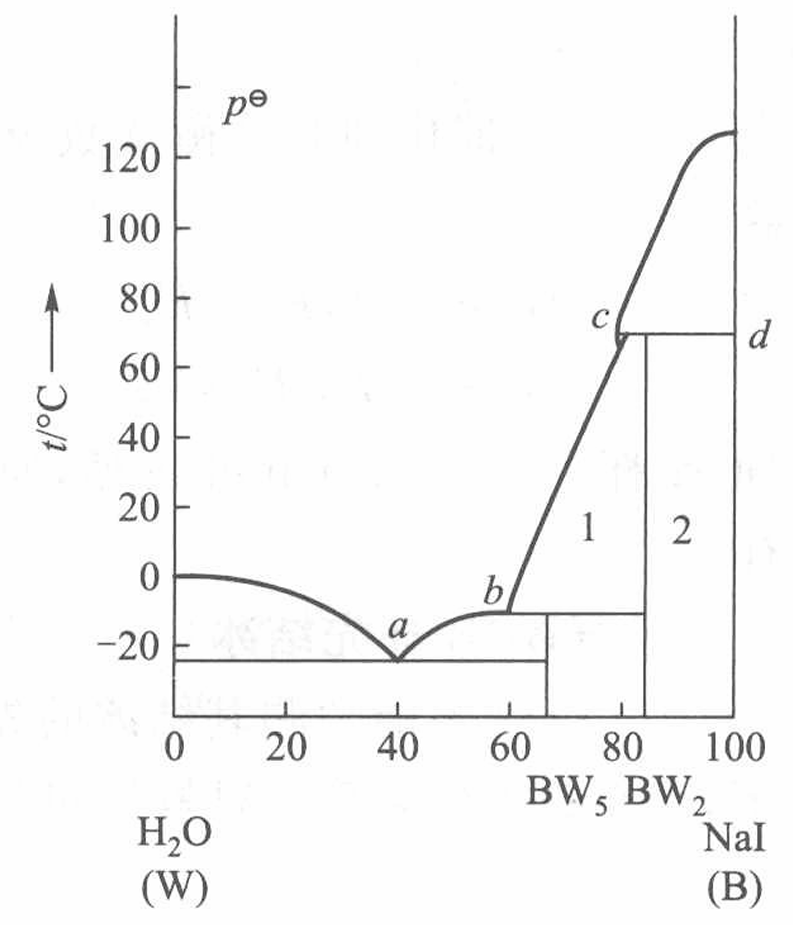
\includegraphics[width=0.52\textwidth]{./Figure/P_2017_5}

\end{figure}

\begin{enumerate}[label=(\arabic*), itemsep=1ex]
    \item 指出$a$、$b$各点的相态、相数与自由度，并说明这些点所代表的意义；
    \item 指出$cd$线，$1$，$2$区的相数、相态与自由度。
\end{enumerate}

\vspace{0.5cm}
\noindent\textbf{六、计算题（15 pts.）}

醋酸酐的分解反应是一级反应，该反应的活化能$E_\mathrm{a}=144348\ \mathrm{J\cdot mol^{-1}}$，已知$284^\circ\mathrm{C}$时，这个反应的$k=3.3\times10^{-2}\ \mathrm{s^{-1}}$，现要控制此反应在$10\ \mathrm{min}$内转化率达到$90\%$，试问反应温度要控制多少摄氏度？

\vspace{0.5cm}
\noindent\textbf{七、计算题（15 pts.）}

电池 $\ce{Pt|H2(g)|HCl(0.01mol\cdot kg^{-1})|AgCl|Ag(s)}$ 的电动势$E/\mathrm{V}=-0.096+1.90\times10^{-3}(T/\mathrm{K})-3.041\times10^{-6}(T/\mathrm{K})^2$，计算$298\ \mathrm{K}$时电池反应的$\Delta_\mathrm{r}G_\mathrm{m}$，$\Delta_\mathrm{r}S_\mathrm{m}$和$\Delta C_{p,\mathrm{m}}$。

\vspace{0.5cm}
\noindent\textbf{八、计算题（20 pts.）}

电池 $\ce{Ag(s)|AgBr(s)|HBr(0.1\ kJ\cdot mol^{-1})|H2(0.01p^\ominus),Pt}$，$298\ \mathrm{K}$时，$E=0.165\ \mathrm{V}$，当电子得失为$1\mathrm{mol}$时，$\Delta_\mathrm{r}H_\mathrm{m}=-50.0\ \mathrm{kJ\cdot mol^{-1}}$，电池反应平衡常数$K^\ominus=0.0301$，$E^\ominus(\ce{Ag+|Ag})=0.800\ \mathrm{V}$，设活度系数均为$1$。
\begin{enumerate}[label=(\arabic*), itemsep=1ex]
    \item 写出电极与电池反应；
    \item 计算$298\ \mathrm{K}$时$\ce{AgBr(s)}$的$K_{\mathrm{sp}}^\ominus$；
    \item 求电池反应的可逆反应热$Q_\mathrm{R}$；
    \item 计算电池的温度系数。
\end{enumerate}